\chapter{Evaluation}

\section{User Evaluation}

\subsection{Data Collection}
Towards the end of this project, I presented \od{} to members~\cite{CfESMembers} of the St Andrews Exoplanet Research Society. This provided an excellent opportunity to get feedback on the software in its current state from its potential users, as well as feature requests and inspiration for future work. To collect this information, I designed a brief artifact evaluation form which is attached as Appendix~\ref{appendix:artifact_eval}. This form covers the main non-functional, user facing requirements of my system. It consists of seven statements with which participants express their agreement by circling the appropriate point on a seven point Likert scale.

The items on the read as follows:
\begin{enumerate}[label=\textbf{it.\arabic*}]
    \item\label{i:gent} The game is entertaining
    \item\label{i:gint} The game interface is intuitive
    \item\label{i:gatt} The game interface is attractive
    \item\label{i:vis} The visualisation interface provides useful controls and visualisations
    \item\label{i:gmint} The game maker interface is intuitive
    \item\label{i:gmuse} The game maker provides useful feedback when making a game\footnote{Due to time restrictions, I was unable to sufficiently present this aspect of the game maker, therefore participants were told to ignore this question and will not include it in my analysis}
    \item\label{i:s} This software would be useful in evaluating human responses to predefined scenarios
\end{enumerate}

\subsubsection{Shortcomings}
The survey is not perfect, here I describe some of its shortcomings:

\begin{enumerate}[label=\textbf{sc.\arabic*}]
    \item\label{sc:acq} I did not take sufficient measures to avoid acquiescence bias\cite{Acquiescence} when designing the form. This is the tendency for users to generally agree with statements, even if this results in two conflicting answers. Avoiding this would have required adding additional, negatively phrased questions in order to establish a baseline level of respondents' agreeableness.
    \item\label{sc:brief} The form is brief, with only seven questions. This was a design decision, made with the aim of increasing engagement. This however, limited the amount of quantitative feedback I received.
    \item\label{sc:int} Participants did not have an opportunity to personally interact with the software, answers provided are based upon a presentation that lasted roughly thirty minutes. I feel that this could particularly impact the questions regarding the intuitiveness of the interface; watching another perform a task they are familiar with can make it seem easier, which may affect one's perception of how intuitive it would be to use themselves.
    \item\label{sc:ex} Responses pertaining to the game UI may have been swayed by the quality of the example game definition I was using. Improving this was not an item of high priority therefore it may not have provided the best demonstration of the framework.
\end{enumerate}
\subsection{Quantitative Analysis}

Since they are categorical, it is not appropriate to average Likert scale data~\cite{LikertAv}. For this reason, I have visualised the results as an aggregated stacked bar chart in figure~\ref{fig:eval_responses}.

\begin{figure}[!h]
    \centering
    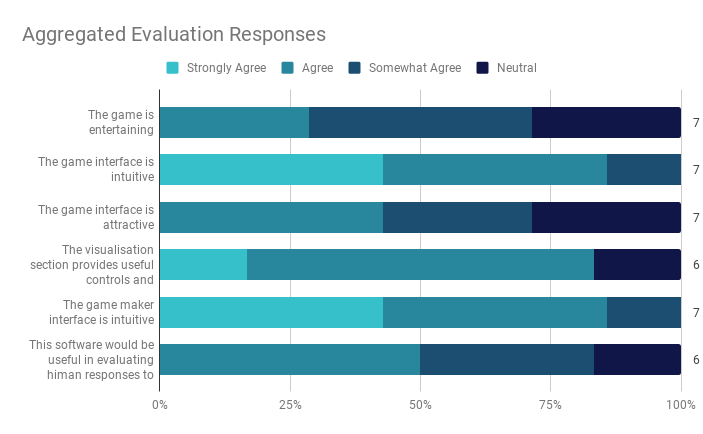
\includegraphics[width=0.9\textwidth]{./images/eval/Aggregated_Evaluation_Responses.png}
    \caption{Visualisation of artifact evaluation likert items. Number to the right of each item indicates the number of responses.}\label{fig:eval_responses}
\end{figure}

From the data, it is immediately striking that none of the responses to any of the items were above 4, meaning that none of them `disagree' to any extent. It is impossible to judge how much of this could be due to acquiescence bias; but I interpret this as a minor effect, due to the extent to which the responses are positive.

Items \ref{i:gent} (entertainment), \ref{i:gatt} (attractiveness) and \ref{i:s} (usefulness) received the lowest levels of agreement. The response to \ref{i:gent} could have been influenced by \ref{sc:ex}, or simply be a deeper comment on the game framework itself. 

\ref{i:gatt} (attractiveness) could be influenced by the images used in this game definition (\ref{sc:ex}), however this aside, in my effort to avoid imposing a bias onto the framework, perhaps achieving a neutral response is desirable here.

\ref{i:s} (usefulness) is intended to provide an assessment of the software as a whole, being used for its intended purpose. This sees agreement, which is a strong sign that the project has been a success. The reasoning for this seeing less agreement than the other items which constitute it could be explained by general thought of doubt around the concept of a game being used to gather player's opinions that were vocally expressed by some participants.

One piece of written feedback was submitted, which stated that it was `very intuitive to create the game'

\subsection{Qualitative Feedback}
The half hour that followed the presentation consisted of discussion around the software and its potential uses.

\subsubsection{Feature Requests}
There were several suggestions to improve various aspects of the software pipeline:

\begin{itemize}
    \item Addition of `sub-decks' - sets of cards which can be easily added or removed in one click, rather than having to select each card manually, possibly multiple times. 
    \item Addition of more than one choice per card.
    \item Addition of an option for pillars to be `invisible'. This would add depth to the games that could be created, allowing for hidden factors that the player can not predict, such as how they are perceived by an enemy.
    \item Addition of game-end condition customisation, for example two pillars must be empty before the game ends, or one must fill.
    \item Addition of different endings, some considered winning and others losing.
\end{itemize}

\section{Objective Evaluation}
\begin{table}[H]
    \begin{tabular}{|p{1.5cm}|p{6cm}|p{1.5cm}|p{6cm}|}
    \hline
    Priority  & Objective                                                                                                                               & Complete?             & Comments                                                                                                                                                                                                                                                                                                \\
    \hline
    Primary   & Devise and implement a game that presents the player with scenarios and allows them to choose from potential responses                  & \cmark&                                                                                                                                                                                                                                                                                                         \\
              & Devise and implement a flexible infrastructure to model and constrain scenarios and their impacts                                       & \cmark&                                                                                                                                                                                                                                                                                                         \\
              & In collaboration with Anne Smith and Christine Helling, devise a sample set of appropriate scenarios with impacts and populate the game & \xmark& Due to the lateness of my first meeting with Anne and Christine, there was not enough time for them to become familiar with the framework and create test scenarios. I did however create my own example scenario.                                                                                      \\
              & Devise and implement an infrastructure for capturing and recording player responses                                                     & \cmark&                                                                                                                                                                                                                                                                                                         \\
              & Implement basic visualisation of responses                                                                                              & \cmark&                                                                                                                                                                                                                                                                                                         \\
    \hline
    Secondary & Devise and implement an admin centre to allow easy creation of new game content                                                         & \cmark& This became a more primary objective, as it became obvious that without the game maker tool, the software would be much less accessible, as technical experience would be required to create new games                                                                                                  \\
              & Carry out an experiment to assess the effectiveness of the game as a tool to assess people's real world views                           & \xmark& It became clear early on that this was a more psychological question, and that I had neither the time or knowledge required to answer this question                                                                                                                                                     \\
              & Create more advanced visualisation and analysis tools                                                                                   & \xmark& After basic visualisations were complete, I prioritised the quality of the game maker tool over more advanced visualisations. The reasoning behind this was that I could not be certain I was providing useful visualisations, and in that case, external tools could be used with the exportable data. \\
    \hline
    Tertiary  & Perform a wider user experiment                                                                                                         & \cmark & This was achieved in the form of the user evaluation forms handed back from members of the Centre for Exoplanet Research.                                                                                                                                                                              \\
    \hline
    \end{tabular}
\end{table}

\section{Future Work}
All of the feature requests raised by participants in the study would make for worthwhile future work, in addition to many other possible quality of life and aesthetic updates. Here I will elaborate on future technical work, as implementation details weren't much discussed in the presentation:

\begin{itemize}
    \item The response system could be expanded and generalised to support different numbers of responses for different cards, rather than two for each.
    \item Depending on the final use case, it may be desirable to add support for collecting user demographic data, such as age and gender. This would require frontend work in making the appropriate forms, as well as increased security for communication (SSL) and encrypted storage on the backend.
    \item Currently the application only deploys locally, some work would be required in implementing a permentant hosting solution. Fortunately this wouldn't be too challenging as this is well documented and supported for Node.
    \item The visualisation tool could be endlessly expanded to become a more capable analysis suite. If more properties to were added to the user data field, there exists the possibility of filtering by age bracket and various other factors.
    \item The game is not currently playabe through any channels other than the site itself. Future work could consist of migrating to a more portable technology, which could be shared and played directly through other channels, such as social media.
    \item Deeper analysis and verification could take place in the game maker. For example, detecting cards that will never be playable given the pillar consequences of choices that must precede them.
\end{itemize}